\documentclass[a4paper, notitlepage]{report}
\begin{titlepage}

\begin{center}

%% Insert the TU Delft logo at the bottom of the page.
\begin{tikzpicture}[remember picture,overlay]
    \node at (current page.south)[anchor=south,inner sep=0pt]{
        
\includegraphics{cover/logo}
    };
\end{tikzpicture}

%% Extra whitespace at the top.
\vspace*{2\bigskipamount}

%% Print the title in cyan.
{\makeatletter
\titlestyle\color{tudelft-cyan}\Huge\@title
\makeatother}

%% Print the optional subtitle in black.
{\makeatletter
\ifx\@subtitle\undefined\else
    \bigskip
    \titlefont\titleshape\LARGE\@subtitle
\fi
\makeatother}

\bigskip
\bigskip

by
%door

\bigskip
\bigskip

%% Print the name of the author.
{\makeatletter
\titlefont\Large\bfseries\@author
\makeatother}

\vfill

in partial fulfillment of the requirements for the degree of
%in overeenstemming met de vereisten voor het verkrijgen van de graad van

\bigskip
\bigskip

{\bfseries Master of Science}

in Applied Physics

\bigskip
\bigskip

at the Delft University of Technology,
%aan de Technische Universiteit Delft,

to be defended publicly on Tuesday January 1, 2013 at 10:00 AM.
%in het openbaar de verdedigen op dinsdag 1 januari om 10:00 uur.

\vfill

\begin{tabular}{lll}
%% Add additional information here, per faculty requirements, e.g
%    Student number: & 1234567 \\
%    Project duration: & \multicolumn{2}{l}{March 1, 2012 -- January 1, 2013} \\
    Supervisor: & Prof.\ dr.\ ir.\ A.\ Einstein \\
    Thesis committee:
        & Prof.\ dr.\ C.\ F.\ Xavier, & TU Delft \\
        & Dr.\ E.\ L.\ Brown, & TU Delft \\
        & Ir.\ M.\ Scott, & Acme Corporation
\end{tabular}

%% Only include the following lines if confidentiality is applicable.
\bigskip
\bigskip
\emph{This thesis is confidential and cannot be made public until December 31, 2013.}
%\emph{Op dit verslag is geheimhouding van toepassing tot en met 31 december 2013.}

\bigskip
\bigskip
An electronic version of this thesis is available at \url{http://repository.tudelft.nl/}.
%Een elektronische versie van dit verslag is beschikbaar op \url{http://repository.tudelft.nl/}.

\end{center}

\end{titlepage}


% All imports needed for file

% General
\usepackage[a4paper,top=1.25in,right=1in,bottom=1.25in,left=1in]{geometry}
\usepackage[utf8]{inputenc}
\usepackage[T1]{fontenc}
\usepackage{textcomp}
\usepackage[bitstream-charter]{mathdesign}
\usepackage{cite}

\usepackage{import}
\usepackage{standalone}
\usepackage{epstopdf}



% Math
\usepackage{amsmath}	% some standard math functions
%\usepackage{amssymb}	% more mathematical symbols
\usepackage{amsbsy}	% enable bold mathematics
\usepackage{bm}
%\usepackage{amsthm}	% enable theorem statements
\usepackage{trfsigns} 	% symbols for transforms

% Text formatting
\usepackage{fancyhdr}	% allow more control over page headers/footers
\usepackage{enumitem}	% allow control over enumerate, itemize, description
\usepackage{setspace}	% allow control over spacing
\usepackage{lastpage}	% provide label for last page in document
\usepackage{sectsty}	% allow control over section styling
\usepackage{url}

% Floats
\usepackage{xcolor}		% enable use of colors
\usepackage{graphicx}		% enable graphics
\usepackage{float}		% enable floats
\usepackage[section]{placeins}	% prevent floats from moving past e.g. sections
\usepackage[small, bf, hang, figurename=Fig.]{caption}	% enable captions for floats (images etc.)
\captionsetup{width=.8\textwidth} % captions not too wide
\usepackage{subcaption}		% enable subcaptions for floats (images etc.)
\usepackage[nottoc]{tocbibind}		% put more stuff in TOC

% Styling data
\pagestyle{fancyplain}

% Title page
\makeatletter
\let\inserttitle\@title
\makeatother

% Page header
\setlength{\headwidth}{\textwidth}
\lhead{} % leave left header empty
\chead{}
\rhead{} % leave right header empty
\lfoot{} % leave left footer empty
\cfoot{} % leave center footer empty
\rfoot{}
\renewcommand{\headrulewidth}{0.3pt}
\renewcommand{\footrulewidth}{0pt}

% Section, equation and figure numbering
\usepackage{chngcntr} 
\counterwithout{figure}{chapter}
\renewcommand{\thechapter}{\Roman{chapter}}
\renewcommand{\thesection}{\Roman{chapter}.\arabic{section}}
\renewcommand{\thesubsection}{\Roman{chapter}.\arabic{section}.\arabic{subsection}}
\renewcommand{\thesubsubsection}{\alph{subsubsection})}
\renewcommand{\thefigure}{\arabic{figure}}
\renewcommand{\thesubfigure}{\alph{subfigure}}
\renewcommand{\theequation}{\thechapter--\arabic{equation}}
\setcounter{tocdepth}{1}
\captionsetup[figure]{labelsep=period}

% Nice enumerations
\newlist{enum}{enumerate}{1}
\setlist[enum]{label=\textbf{[\arabic*]}} % \arabic or \alpha
\setlist{itemsep=-5pt}

% Nice \begin{StateDescription} for FSM descriptions
\newlist{StateDescription}{description}{1}
\setlist[StateDescription]{font=\normalfont\scshape, labelwidth=12em, leftmargin=12em,listparindent=0em,itemindent=0em}

% Section formatting
\definecolor{title-gray}{gray}{0.45}		% grijstint voor headers
\renewcommand*\sfdefault{lmss}
\allsectionsfont{\sffamily\color{title-gray}}	% sans-serif in headers

% Page layout
\onehalfspacing					% Wide margins for text
\usepackage{chngpage}			% customize margins of certain pages
\usepackage{adjustbox}

% Text macros
\usepackage{xspace}
\newcommand{\matlab}{MATLAB\xspace}		% fancy MATLAB command
\newcommand{\norm}[1]{\left\lVert#1\right\rVert}% Command for vector norm
\newcommand{\abs}[1]{\left\lvert#1\right\rvert}% Command for abs
\newcommand{\todo}[1]{\textbf{\textcolor{red}{#1}}}	% placeholder stuff
\let\oldhat\hat
\renewcommand{\vec}[1]{\bm{#1}} % bold vectors in math mode
\newcommand{\vechat}[1]{\oldhat{\bm{#1}}} % hat in vector mode
\newcommand{\mat}[1]{\bm{#1}} % bold matrix in math mode

%links
\usepackage{hyperref}
\hypersetup{ %setup hyperlinks
    colorlinks=true,
    citecolor=black,
    filecolor=black,
    linkcolor=black,
    urlcolor=black
}

\begin{document}

\section{Simulation}
\label{sec:sync-simulation}
To characterize the performance of just the synchronization subsystem, a simulation was constructed that measures the error of the estimate $\hat{\tau}$ in different scenarios. This simulation is performed for different values of synchronization delay, reverberation and signal-to-noise ratio.

\subsection{Scope and implementation}
First, the simulation generates the MLS signal that is used for all simulations. Based on this, a number of microphone signals are generated. Each signal is convolved by $K$ different FIR filters, each representing a room impulse response for a 5 by 6 by 2.5 metre cuboid-shaped room with a variable wall acoustic reflection coefficient\footnote{These FIR filters were computed by the rir.m file available from the \matlab Central File Exchange at \url{https://www.mathworks.com/matlabcentral/fileexchange/5116-room-impulse-response-generator/content/rir.m}}. Each of these signals is delayed by $L$ different delays, yielding a $K \times L$ set of convolved and delayed sample signals.

Then, for each delay and reflection value, $M$ different signal-to-noise ratios are evaluated. For each SNR, $N$ realizations of Gaussian noise at that magnitude are generated so that, in total, $K \times L \times M \times N$ simulation runs were performed. This noise realization is added to the pre-generated sample signal and both the time- and frequency-domain correlation algorithms described above are run on this noisy signal. The difference between the actual inserted delay and the estimated delay is computed and stored in a result vector.

The parameters used for this simulation are as follows: $K = 10$ different wall reflection coefficients from 0 to 1 (unitless), $L = 10$ different delays from $0~\mathrm{s}$ to $0.2~\mathrm{s}$, $M = 20$ different noise signal-to-noise ratios from $60~\mathrm{dB}$ to $-34~\mathrm{dB}$ and $N = 100$ noise realizations for each parameter combination.

\subsection{Expected results}
Due to the favorable properties of the beacon signal described in \ref{sec:mls}, it is expected that the time-domain algorithm will be robust in the face of introduced noise. As this algorithm relies on finding a global maximum in the impulse response, however, it is suspected that for high values of wall reflectance, combined with multipath interference, a maximum in the impulse response might arise that does not correspond to the direct acoustic path. This would lead to a large estimation error beyond a certain critical wall reflection coefficient. In addition, the time-domain algorithm is only accurate to integer samples, leading to an expected round-off error of less than one sample.

The frequency-domain algorithm is expected to provide sub-sample accuracy due to its least-squares estimation of the delay in the frequency domain. However, performance is reliant on low phase contribution of the acoustic impulse response compared to the contribution of the delay that must be estimated (equation \ref{eq:rir-influence-fd}). It is unknown whether this assumption will hold throughout the simulation scenarios.

It is not expected that the performance of either algorithm will depend on the amount of introduced delay.

\subsection{Results}
The reflection coefficient has no influence on the performance of the time-domain algorithm, but the frequency-domain algorithm is crippled at reflection values of $0.8$ or higher (Fig.~\ref{fig:sync-simulation-reflection}). The frequency-domain algorithm is much more susceptible to noise than the time-domain algorithm (fig \ref{fig:sync-simulation-noise}). Neither algorithm is affected by the amount of delay (fig \ref{app:sync-simulation-delay} in the appendix). A discussion of the results may be found in section \ref{sec:disc_to}.

\begin{figure}[H]
\begin{adjustwidth}{-1in}{-1in}
\centering
	\begin{subfigure}{0.5\textwidth}
		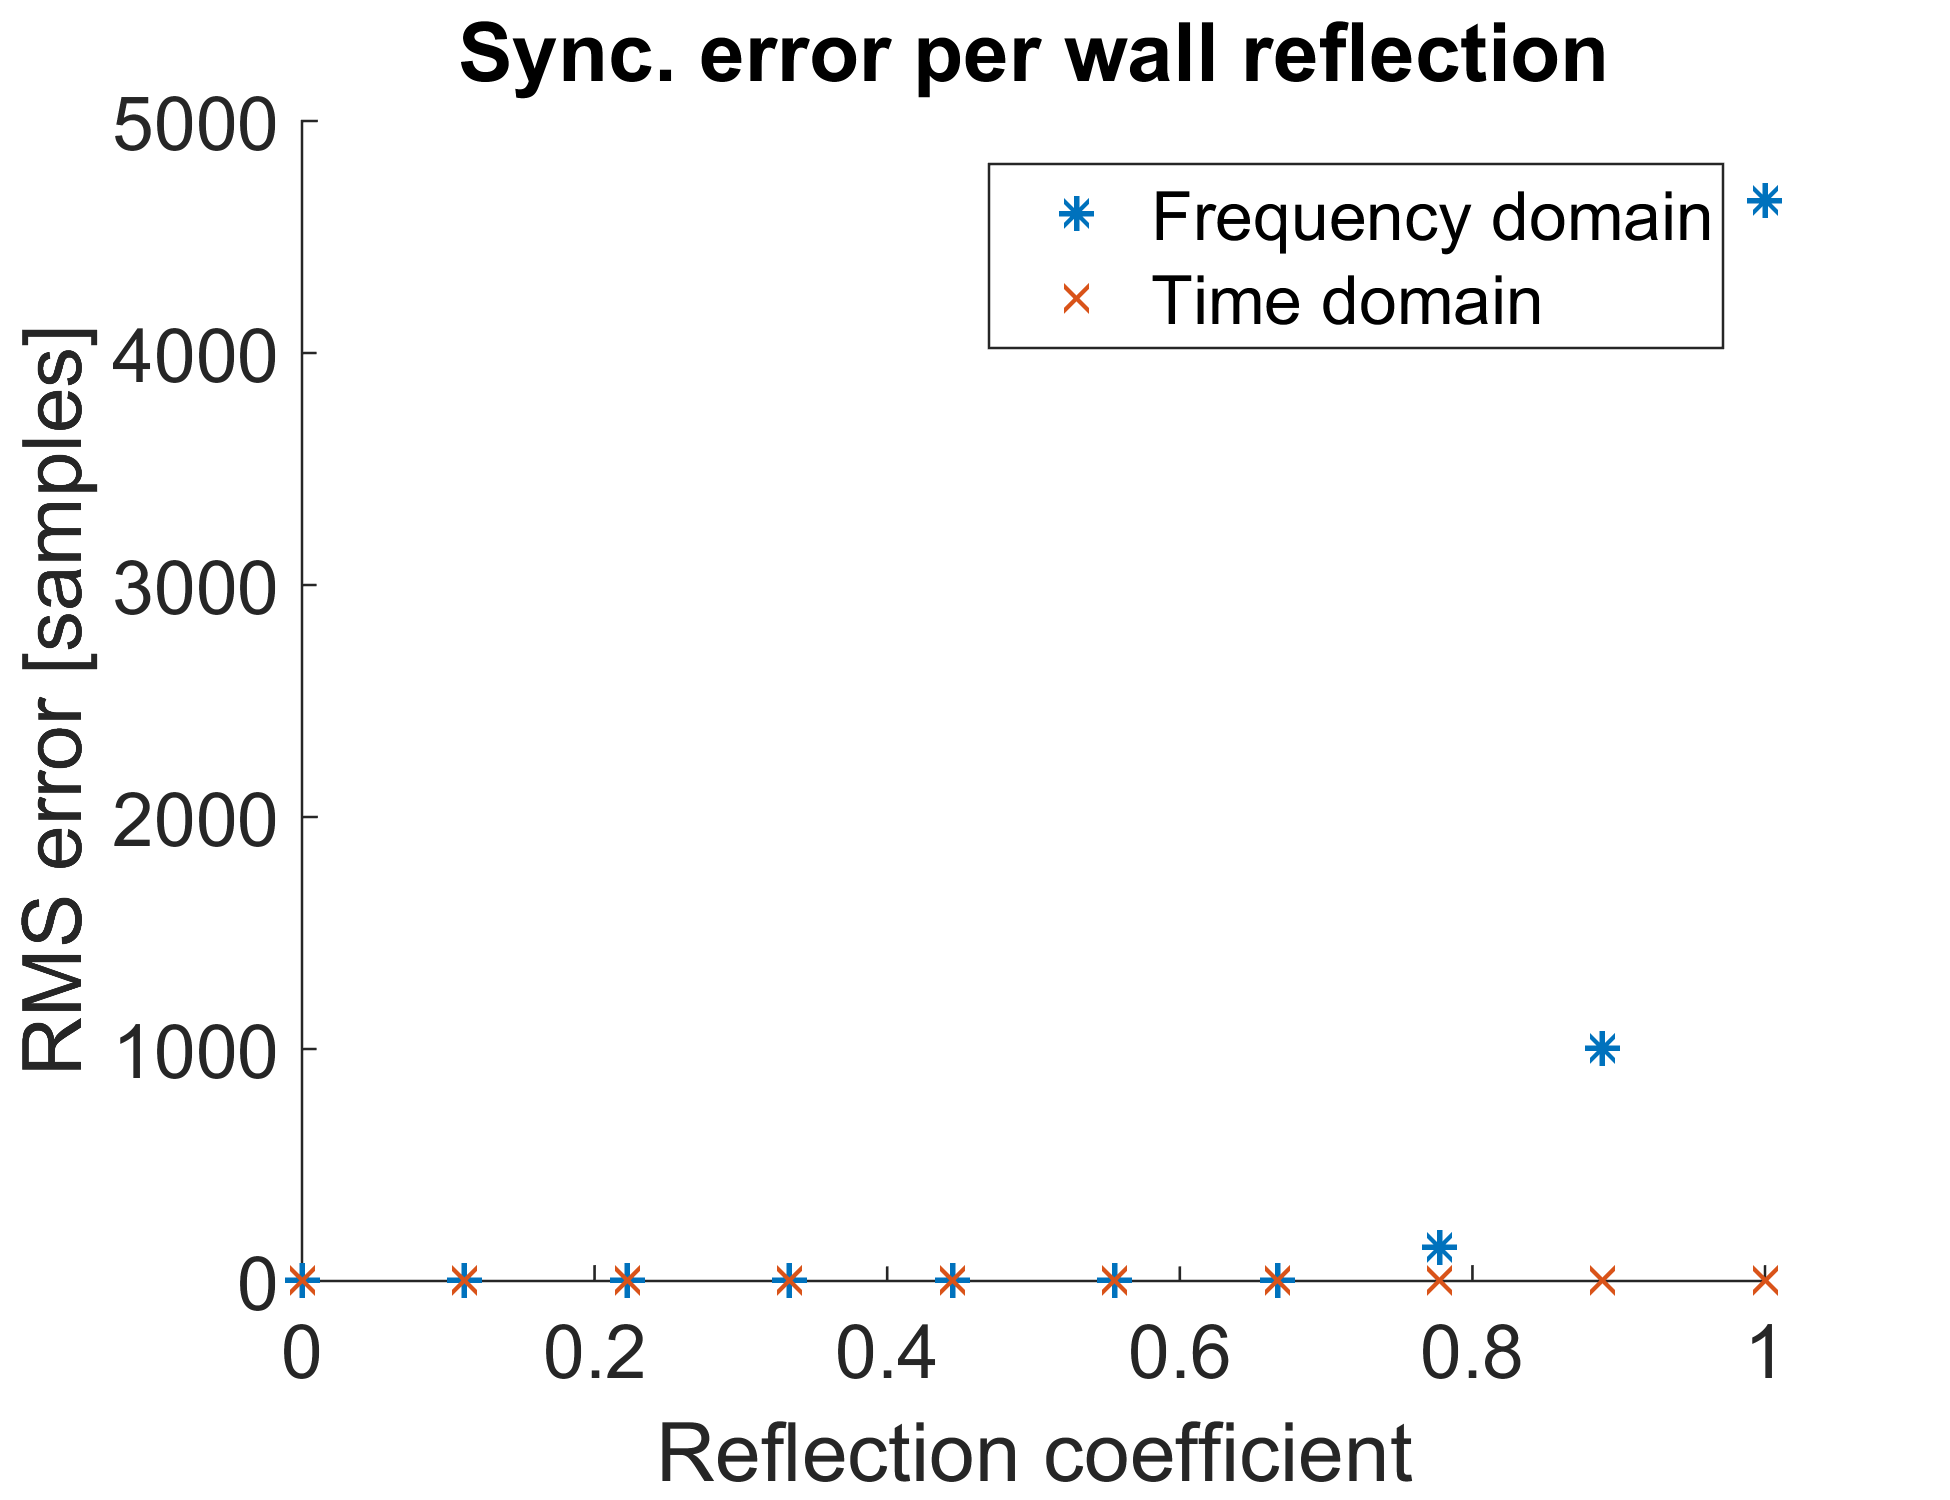
\includegraphics[width=\textwidth]{figures/sync-simulation/error-vs-reflection}
		\caption{Delay estimation error as a function of wall reflection.}
		\label{fig:sync-simulation-reflection}
	\end{subfigure}
	\begin{subfigure}{0.5\textwidth}
		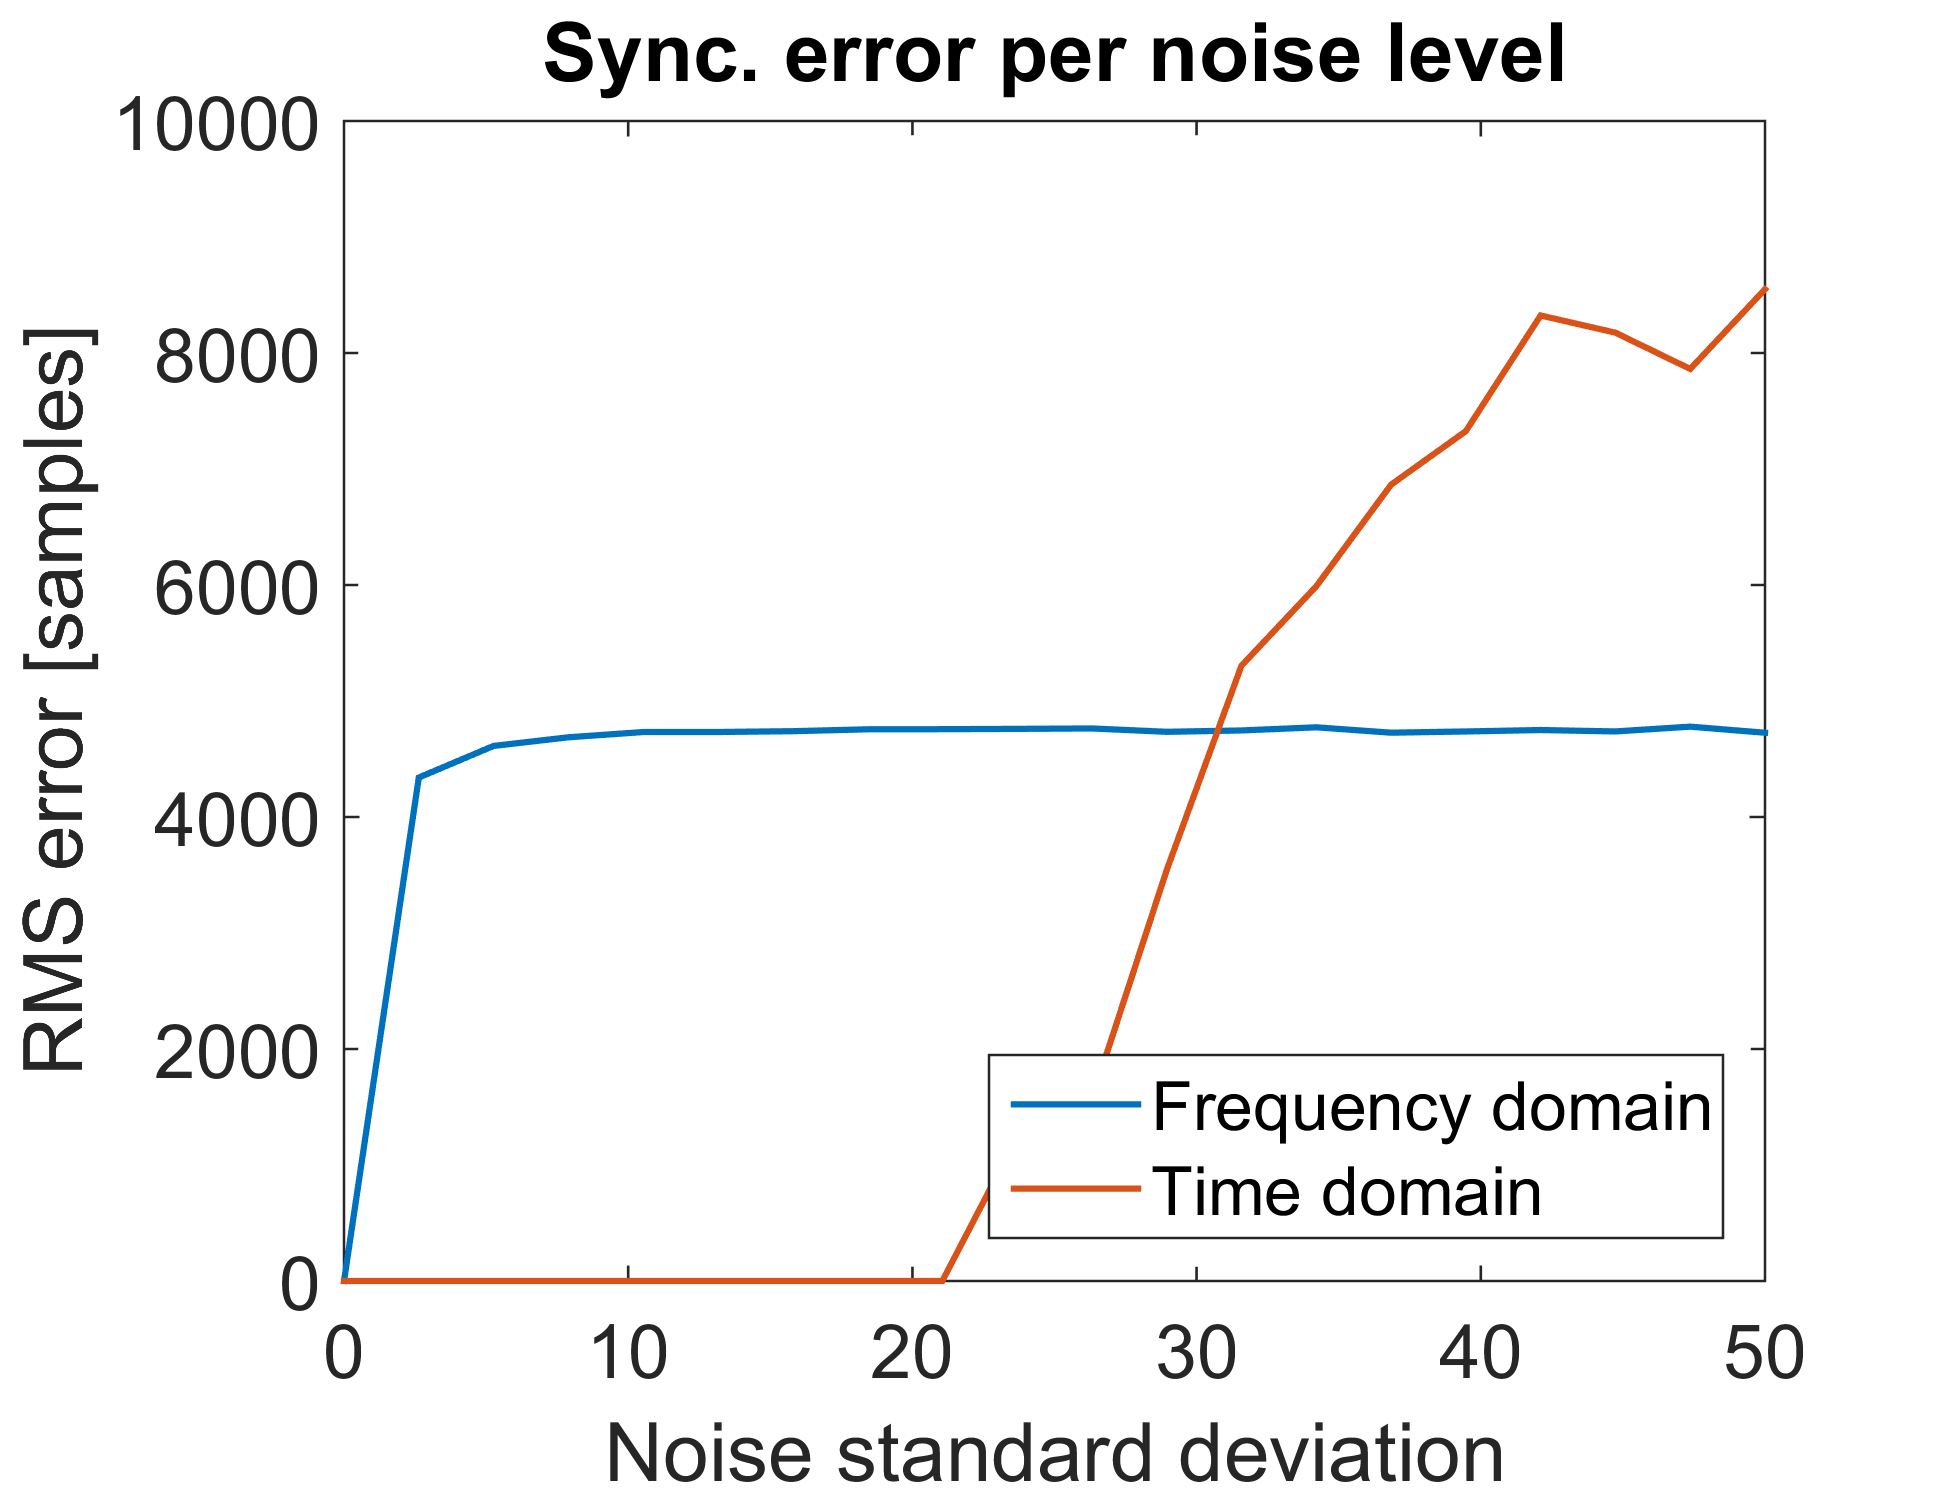
\includegraphics[width=\textwidth]{figures/sync-simulation/error-vs-noise}
		\caption{Delay estimation error as a function of noise power}
		\label{fig:sync-simulation-noise}
	\end{subfigure}
\end{adjustwidth}
\caption[TD and FD synchronization simulation results.]{Simulated results for TD and FD synchronization algorithm.}
\label{fig:sync-simulation}
\end{figure}


\end{document}
